\documentclass{article}
\usepackage[utf8]{inputenc}
\usepackage[spanish]{babel}
\usepackage{listings}
\usepackage{graphicx}
\graphicspath{ {images/} }
\usepackage{cite}

\begin{document}

\begin{titlepage}
    \begin{center}
        \vspace*{1cm}
            
        \Huge
        \textbf{La memoria del computador}\par
        \vspace{0.5cm}
        \LARGE
        \text{Informática II}
        \vspace{1.5cm}
            
        \textbf{Angee Lorena Ocampo Ramírez}
            
        \vfill
            
        \vspace{0.8cm}
            
        \Large
        Departamento de Ingeniería Electrónica y Telecomunicaciones\\
        Universidad de Antioquia\\
        Medellín\\
        Septiembre de 2020
            
    \end{center}
\end{titlepage}

\tableofcontents\newpage

\section{Introducción}
En este documento se brindará una descripción al lector de todo lo referente a a la memoria , los tipos de memorias que hay en el computador, cómo funciona, como se gestiona; todo esto con el objetivo de explicar la importancia de la memoria en el computador.\par

\section{Contenido} \label{contenido}
\subsection{¿Qué es la memoria del computador?}\par
Es un dispositivo que guarda y almacena la información usada por el usuario para ser procesada por el computador.
\subsection{Mencione los tipos de memoria que conoce y haga una breve descripción de cada tipo}\par
\textbf{Memoria ROM:}(Read Only Memory),esta emoria solo le sirve al computador al principio, ya que esta memoria solo sirve para la lectura como su nombre lo indica, por lo tanto, se convierte en la guía del computador en el inicio de su vida útil, puesto que tiene las BIOS, entre otros elementos necesarios para comenzar su funcionamiento.\par

\textbf{Memoria RAM:} (Random acces memory),esta es la memoria más importante del computador, ya que en esta se guarda toda la información necesaria para ser procesada.Además,al ser más rápida que el disco duro permite un acceso más eficiente.\par

\textbf{Memoria Caché:}En este memoria se almacena los datos que se usan con mayor frecuencias, todo esto con el objetivo de permitir al usuario un acceso más veloz.\par

\subsection{Describa la manera como se gestiona la memoria de un computador}\par
El usuario da la misión a completar, después, el microprocesador se dirige al disco duro y carga todo la información que hay de la aplicación o archivo a la memoria RAM, puesto que esta es mucho más veloz que el disco duro y permitirá que el microprocesador obtengo un acceso inmediato a los datos de la aplicación o archivo.\par
Luego, el microprocesador comenzará a ejecutar una y otra vez las instrucciones dadas por la RAM hasta que la tarea haya sido completada; cuando esto pasa, se eliminarán las ordenes e información ya ejecutada para dar paso a otros datos o no gastar más memoria de forma innecesaria; además, el microprocesador guardará todos los cambios hechos en el disco duro, debido a que este es <<un dispositivo de almacenamiento permanente>> \cite{Salazar} para que no se pierdan para siempre.\par
Toda esta gestión se hace con el fin de administrar la memoria principal, con la asignación de esta memoria a los procesos que se solicitan, localizando los espacios ocupados y libre en la memoria, cargando la información a esta para que los programas y archivos funcionen, además, de utilizar al máximo la memoria principal del computador,entre otras funciones. Esta gestión está enteramente ligada a la arquitectura del computador.\cite{Rosenberg}

\begin{figure}[h]
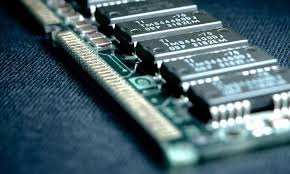
\includegraphics[width=6cm]{descarga.png}
\centering
\caption{Memoria\cite{Anonimo}}
\label{fig:cpplogo}
\end{figure}

\subsection{¿Qué hace que una memoria sea más rápida que otra? ¿Por qué esto es importante?}\par
Hay demasiados factores que pueden entrar a jugar a la hora de determinar la velocidad de la memoria; por ejemplo,la capacidad de la memoria RAM pero solo si esta ya ha sido utilizada por el procesador completamente, ya que al no tener más de esta memoria comienza a usar el disco duro, que es mucho más lento, como extensión de la memoria RAM.Esto provoca que el funcionamiento de la máquina sea mucho más lento.\par
Otro causa, es el bus de control, puesto que <<establece la frecuencia o ritmo de trabajo en la que se comunican ambos dispositivos>>\cite{Salazar}.También influye la latencia que el <<tiempo que transcurre entre una petición y su respuesta>>\cite{breixobaloca}, por eso, entre menor sea este tiempo más rápido será el proceso y la memoria.\par
Por último está el disco duro, ya que en este están almacenados todos los elementos; como, sistemas operativos, documentos, música, etc; y la velocidad con la que el microprocesador acceda al disco duro hará que el proceso sea rápido o lento.\cite{El_Comercio}\par
Este aspecto de la velocidad de la memoria es muy importante porque hace que los procedimientos realizados por la computadora sean más eficientes, asimismo, de esta velocidad depende que el procedimiento sea útil o no. Igualmente, si los procedimientos se realizan de una forma más rápida habrá un ahorro de tiempo que en el contexto de la solución de problemas en la vida real puede significar muchas cosas, como brindarme el resultado de una operación que se necesita con urgencia, entre otras.\par

\section{Conclusión} \label{conclulsion}
Todo esto evidencia el papel tan importante que juega la memoria en el procesamiento de datos; ella defina los límites y la capacidad de la máquina; además de su buen funcionamiento depende la culminación de la tarea a realizar. También, deja en claro que su agilidad y alcance pueden mejorar o empeorar el rendimiento de la máquina.

\bibliographystyle{IEEEtran}
\bibliography{references}

\end{document}
